\chapter{IPv6-Neighbor Discovery}
\label{chap:ipv6_nd}

\section{Ejercicio 4.1}
\subsection{¿Por qué es necesario el NS que se envía en t = 6 s? Muestra una captura del log del nodo que lo envía que muestre el motivo del envío. ¿Qué paquete cumple la misma función en IPv4?}

\begin{figure}[H]
    \centering   
    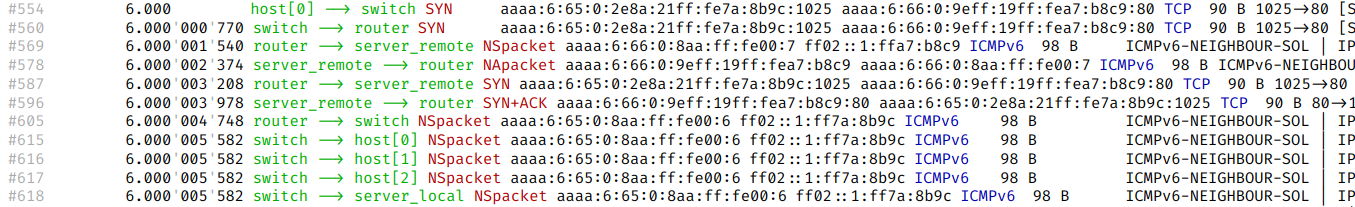
\includegraphics[width=135mm, scale=0.75]{imaxes/captura_ejer4_1.png}
    \caption{Ventana logs paquete NS en t=6s}
    \label{fig:logs_ns_t6}
\end{figure}

Como se puede ver en la imagen \ref{fig:logs_ns_t6}, el nodo que envía el paquete Neighbor Solicitation en t=6s es el router. El host[0] empieza la conexión mandando un SYN al servidor remoto pero como no tiene información de su MAC, el router manda al servidor un NS para asi averiguar su MAC ya que solamente le llega una IP pero no sabe a que dispositivo le corresponde. Esto ocurre ya que, al no existir una entrada en la Neighbor Cache para el serverRemote, el dispositivo debe enviar un mensaje NS para solicitar esa información a través del protocolo Neighbor Discovery.

En el caso de IPv4, el mensaje que realiza una función similar al NS (Neighbor Solicitation) de IPv6 es el mensaje de solicitud ARP (ARP Request). Tanto el NS en IPv6 como la solicitud ARP en IPv4 se utilizan para descubrir la dirección física (de la capa de enlace) que corresponde a una dirección IP o de red específica.

\section{Ejercicio 4.2}
\subsection{¿Por qué no se usa una IP unicast para ese mensaje, si ya es conocida?}

No se utiliza la dirección unicast aunque sea conocida ya que en IPv6 se emplea una dirección de multicast especial para la resolución de direcciones. Esto se hace para evitar enviar el mensaje a todos los dispositivos de la red. Esta dirección multicast es escuchada solo por el dispositivo que posee la dirección de destino, limitando el tráfico de resolución de direcciones a los dispositivos interesados y asi no sobrecargar la red, ganando asi eficiencia y recursos.


\section{Ejercicio 4.3}
\subsection{Muestra capturas de la neighbor cache del nodo que envió el NS un segundo antes de enviarlo, justo después de enviarlo pero antes de recibir el paquete de respuesta y justo después de recibir la respuesta y explica las diferencias entre los 3 estados. (Nota: para ver la neighbor cache haz doble click sobre el nodo → ipv6 → neighborDiscovery, y a continuación expande owned objects en la ventana inferior izquierda. La neighbor cache es el atributo neighbourMap.)}


\begin{enumerate}
    \item Un segundo antes de enviar el NS
    
    \begin{figure}[H]
        \centering
        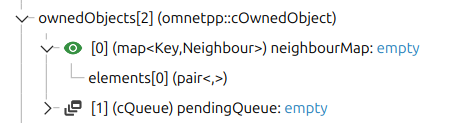
\includegraphics[width=135mm, scale=0.75]{imaxes/captura_ejer4_33.png}
        \caption{Neighbor cache del router antes de enviar NS}
        \label{fig:paquete_antes_t6}
    \end{figure}

    En este momento, la neighbor cache del router está vacía ya que en ningún momento tuvo que mandar un paquete IPv6 al servidor remoto, por lo que no necesitó nunca guardar su dirección MAC.

    \item Justo después de enviar el paquete NS
    
    \begin{figure}[H]
        \centering
        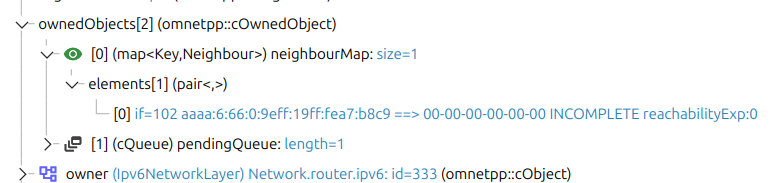
\includegraphics[width=135mm, scale=0.75]{imaxes/captura_ejer4_31.png}
        \caption{Neighbor cache del router después enviar NS}
        \label{fig:paquete_ns_t6}
    \end{figure}

   Como se puede ver en la imagen \ref{fig:paquete_ns_t6}, el estado de la entrada de la neighbor cache del router es el estado INCOMPLETE tras haber enviado un mensaje NS ya que al querer enrutar el paquete SYN que envió el host[0], tiene que averiguar la MAC de la IP destino, por lo que está a la espera de la respuesta de la MAC del servidor. En la entrada tiene como destino la IP global del servidor remoto y la MAC asociada es la 00:00:00:00:00:00 ya que no la sabe

    \item Un segundo después de enviar el paquete NS
    \begin{figure}[H]
        \centering
        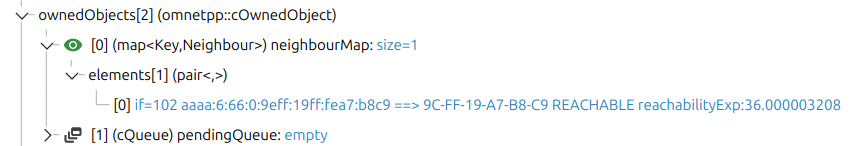
\includegraphics[width=135mm, scale=0.75]{imaxes/captura_ejer4_32.png}
        \caption{Neighbor cache del router al recibir respuesta del paquete NS}
        \label{fig:respuesta_ns_t6}
    \end{figure}

    Como se puede ver en la imagen \ref{fig:respuesta_ns_t6}, el estado de la entrada de la cache del router pasa a ser REACHABLE ya que se recibió la respuesta indicando que es una dirección alcanzable. También se puede ver que en la entrada de la caché ya aparece la MAC del servidor mapeada con su dirección IPv6 

\end{enumerate}



\section{Ejercicio 4.4}
\subsection{¿Envía el host[1] algún otro mensaje NS después del instante t = 6 s? ¿Cuál es su objetivo? Muestra una captura del mensaje en Wireshark y una captura del log en la que se muestre el motivo del envío.}

En la figura \ref{fig:postNShost0}, se observa que host[0] vuelve a enviar un paquete de NS en t = 11 (También se repite en t = 47, y así sucesivamente). El motivo del envío, es la finalización del NUD (Neighbor Unreachability Detection), como refleja la figura \ref{fig:NS_purpose}. Este timeout define el tiempo que pasa en DELAY la entrada de la dirección unicast del router en la tabla de caché de neighborDiscovery de host[0] (Normalmente 5s).

\begin{figure}[H]
    \centering
    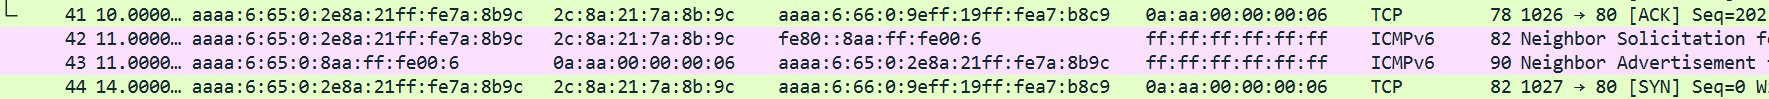
\includegraphics[width=135mm, scale=0.75]{imaxes/ejercicio4_4_1.png}
    \caption{Intercambio de NS y NA entre host[0] y Router}
    \label{fig:postNShost0}
\end{figure}

\begin{figure}[H]
    \centering
    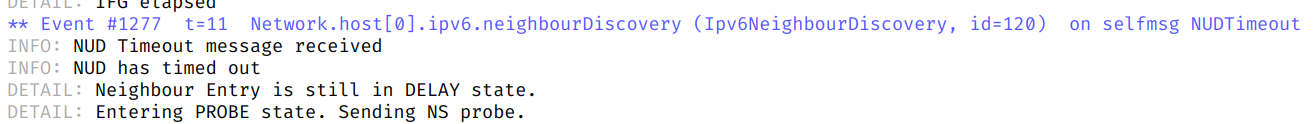
\includegraphics[width=135mm, scale=0.75]{imaxes/ejercicio4_4_2.png}
    \caption{Motivo del envío del Ns}
    \label{fig:NS_purpose}
\end{figure}

\section{Ejercicio 4.5}
\subsection{¿Es la IP destino de este NS del mismo tipo que en los NS enviados anteriormente? ¿Por qué?}

La IP de destino en el NS en t=11 está en formato unicast link-local, diferenciándose este paquete de los enviados anteriormente en la simulación, que se enviaban a multicast de nodo solicitado. Esto, es debido a que ahora host[0] sí conoce la dirección del router, simplemente quiere saber si está activo y en la misma dirección que host[0] conoce. Las direcciones multicast se necesitan cuando se quiere enviar un mensaje a varios nodos, que no es el caso en esta situación.


\section{Ejercicio 4.6}
\subsection{Muestra capturas de la neighbor cache del host[1] en los siguientes instantes de tiempo:}

\begin{enumerate}
    \item 7 segundos antes del envío del NS de la pregunta anterior.
    \begin{figure}[H]
        \centering
        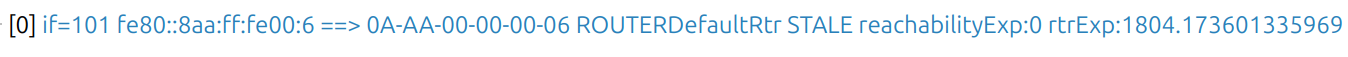
\includegraphics[width=135mm, scale=0.75]{imaxes/ejercicio4_5_1.png}
        \caption{Estado de la tabla en t=4 (La ruta al router comienza en estado STALE)}
        \label{fig:51}
    \end{figure}
    \item 3 segundos antes del envío del NS.
    \begin{figure}[H]
        \centering
        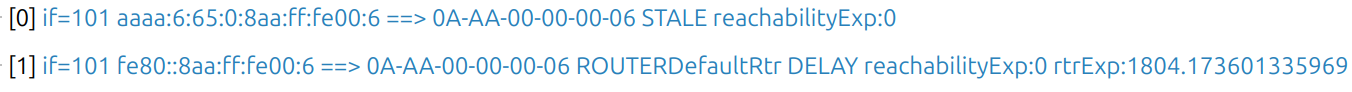
\includegraphics[width=135mm, scale=0.75]{imaxes/ejercicio4_5_2.png}
        \caption{Estado de la tabla en t=10 (La ruta pasa a estado DELAY hasta que pasen 5 segundos o se reciba un paquete de esa dirección)}
        \label{fig:52}
    \end{figure}
    \item Justo después del envío del NS y antes de recibir el NA respuesta.
    \begin{figure}[H]
        \centering
        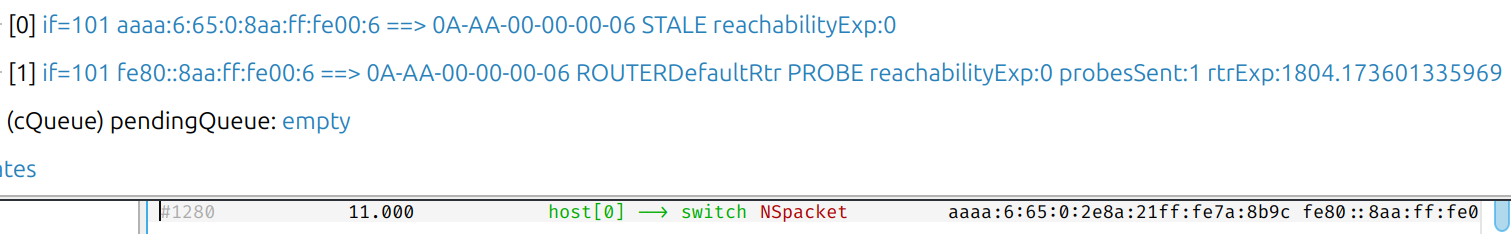
\includegraphics[width=135mm, scale=0.75]{imaxes/ejercicio4_5_3.png}
        \caption{Estado de la tabla en t=11, tras el envío del NS (La ruta pasa a estado PROBE y se mantendrá ahí hasta que se lleve a cabo el intercambio de paquetes NS y NA)}
        \label{fig:53}
    \end{figure}
    \item Justo después de recibir el NA respuestas
    \begin{figure}[H]
        \centering
        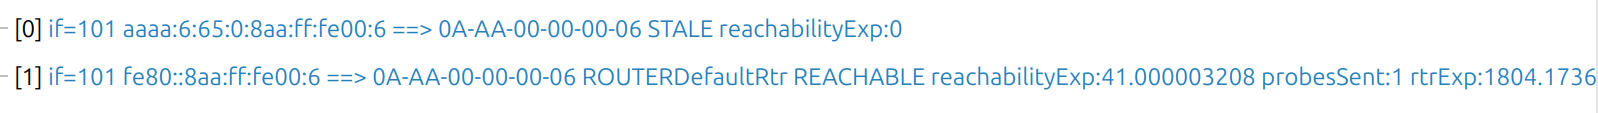
\includegraphics[width=135mm, scale=0.75]{imaxes/ejercicio4_5_4.png}
        \caption{Estado de la tabla en t=11, tras el envío del NA (La ruta pasa a estado Reachable, porque el router contesta con el NA)}
        \label{fig:54}
    \end{figure}
\end{enumerate}
